\begin{figure}[!h]
  \setlength{\unitlength}{\textwidth}

  \begin{picture}(1,1.2)(0,0)
    % % %90
      % % % Parkinson Data 
      \put(0.005,0.8){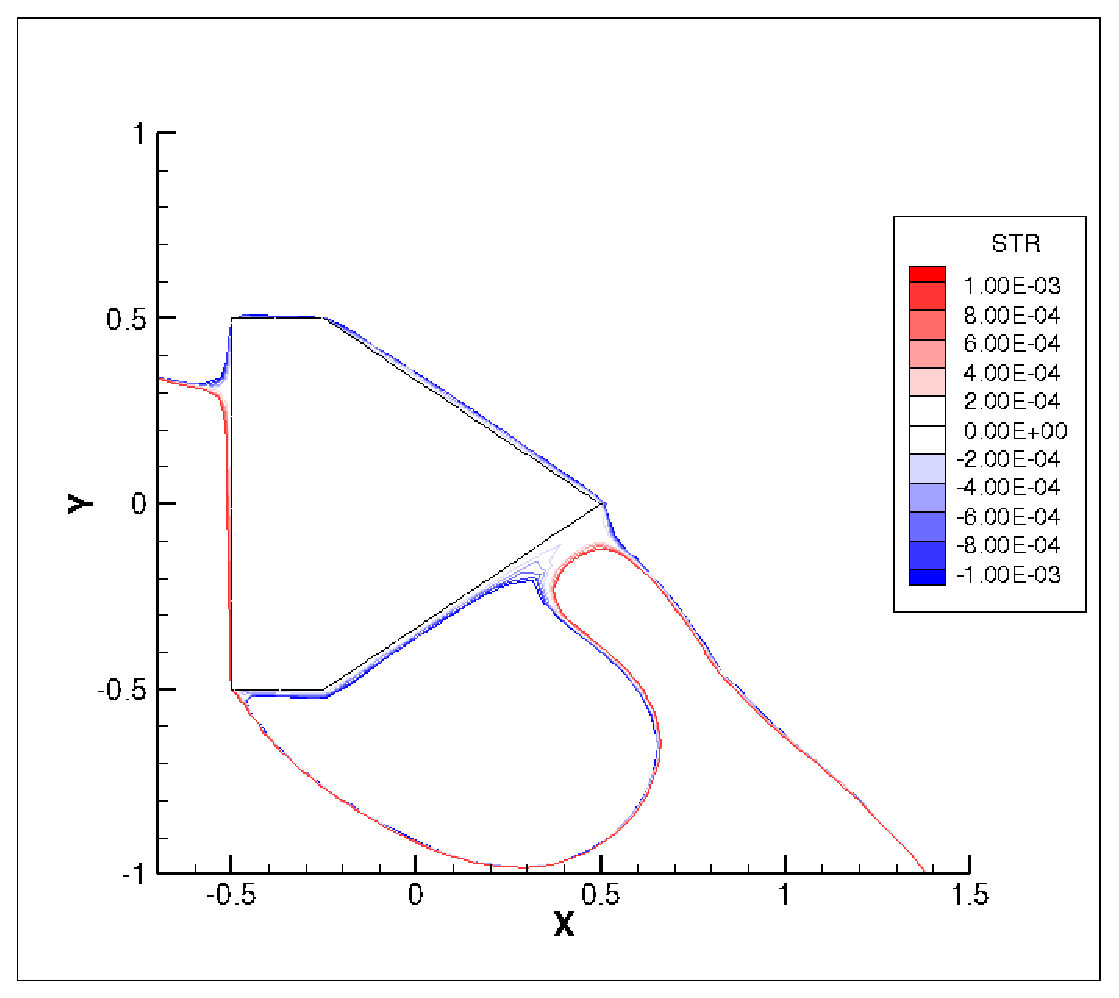
\includegraphics[width=0.4\unitlength]{./chapter-cross-sections/fnp/fsi-0.25-1.eps}}
      \put(0.005,0.4){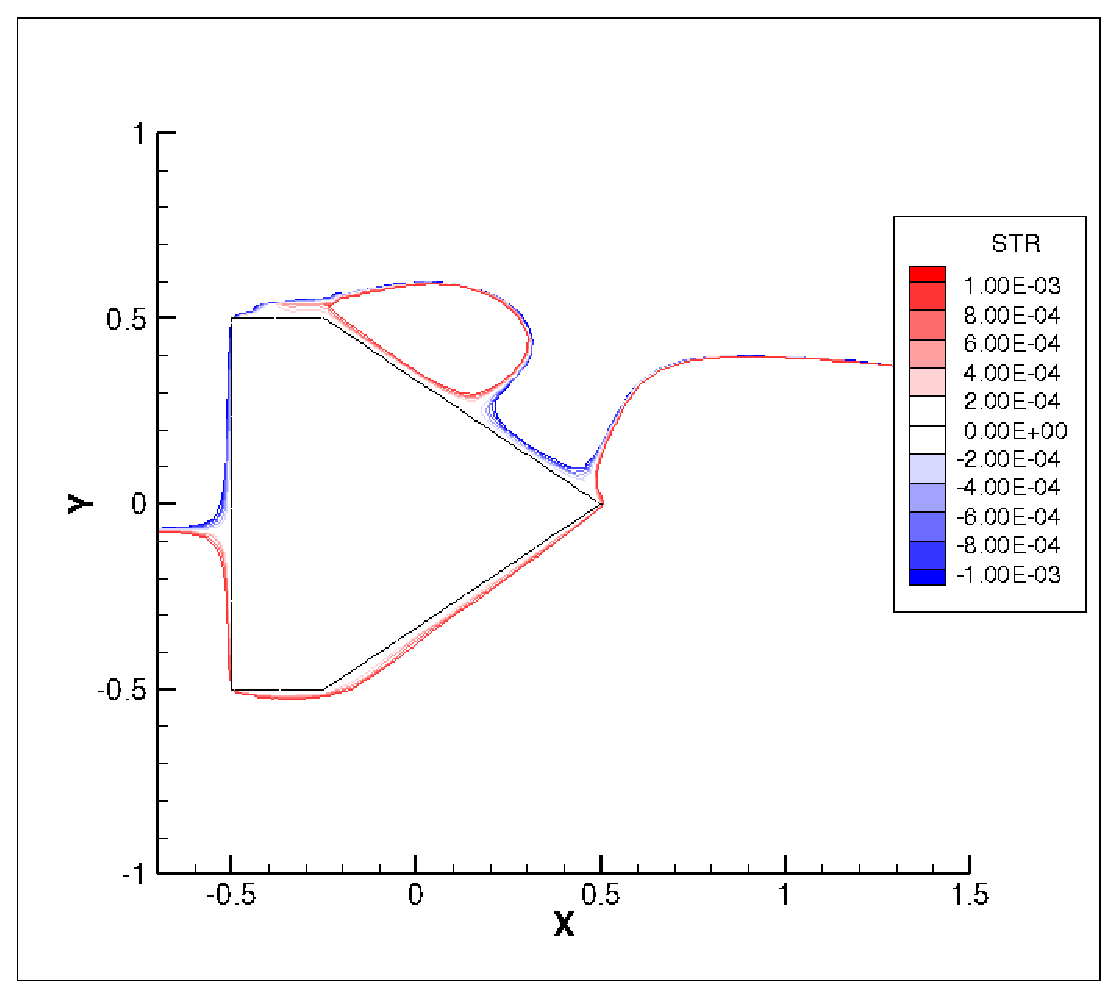
\includegraphics[width=0.4\unitlength]{./chapter-cross-sections/fnp/fsi-0.25-2.eps}}
      \put(0.005,0.0){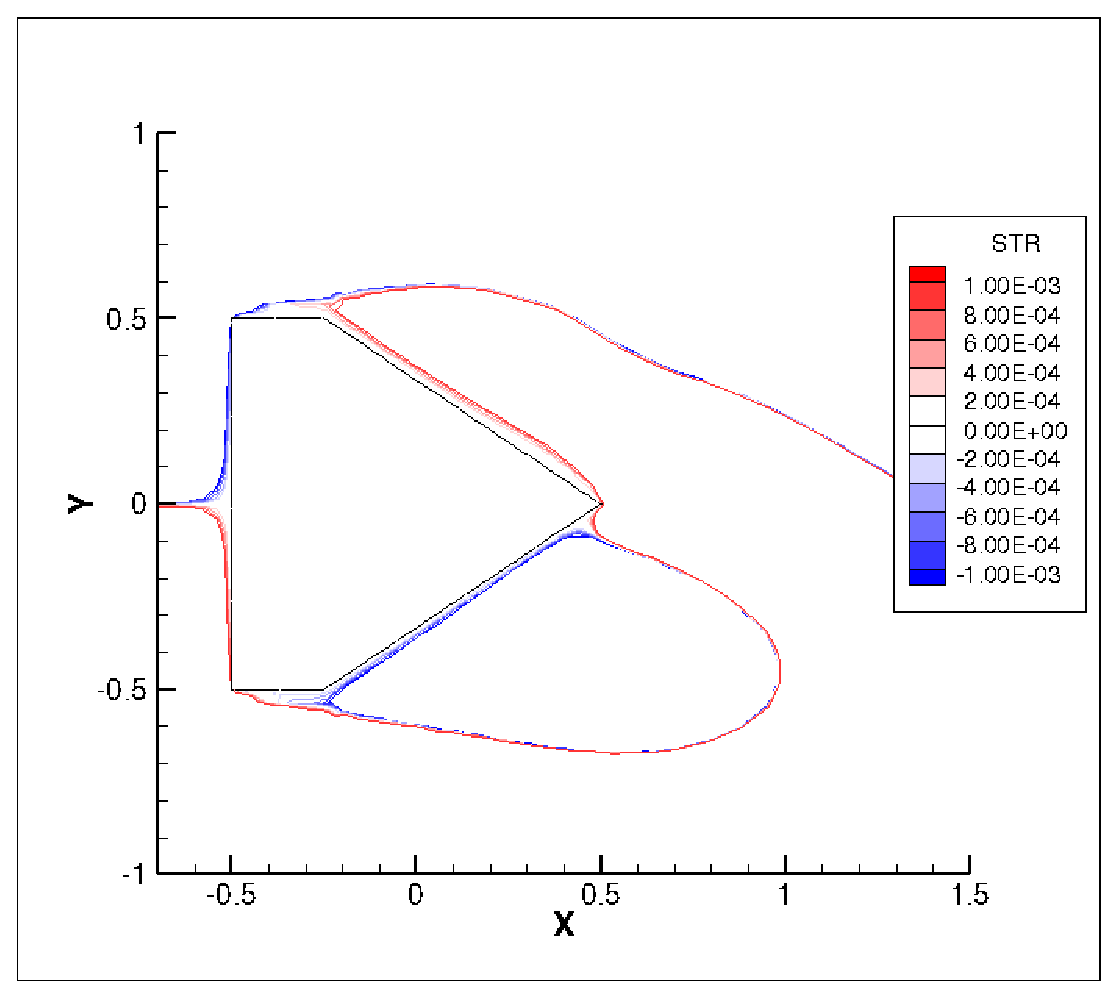
\includegraphics[width=0.4\unitlength]{./chapter-cross-sections/fnp/fsi-0.25-3.eps}}

      
      
      \put(0.505,0.8){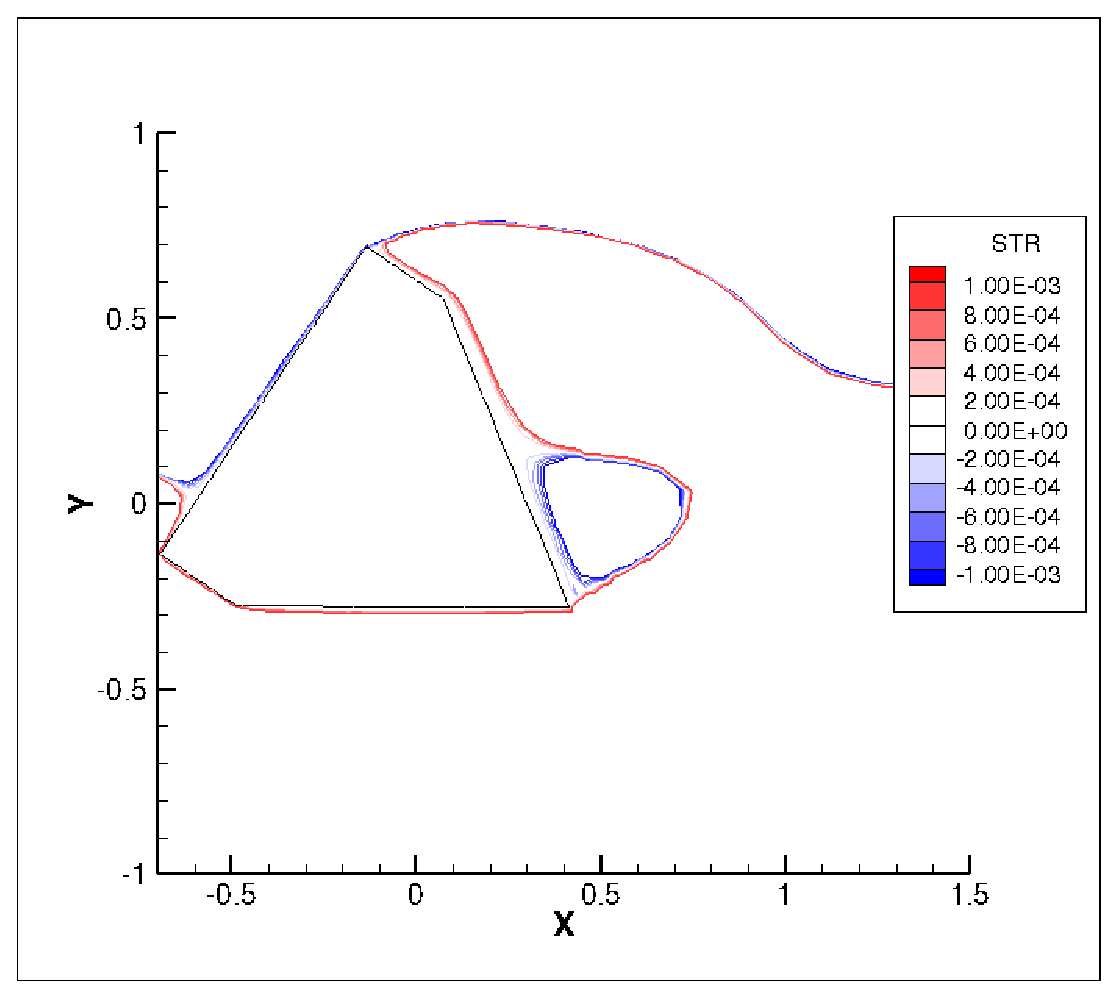
\includegraphics[width=0.4\unitlength]{./chapter-cross-sections/fnp/qss-0.25-1.eps}}
      \put(0.505,0.4){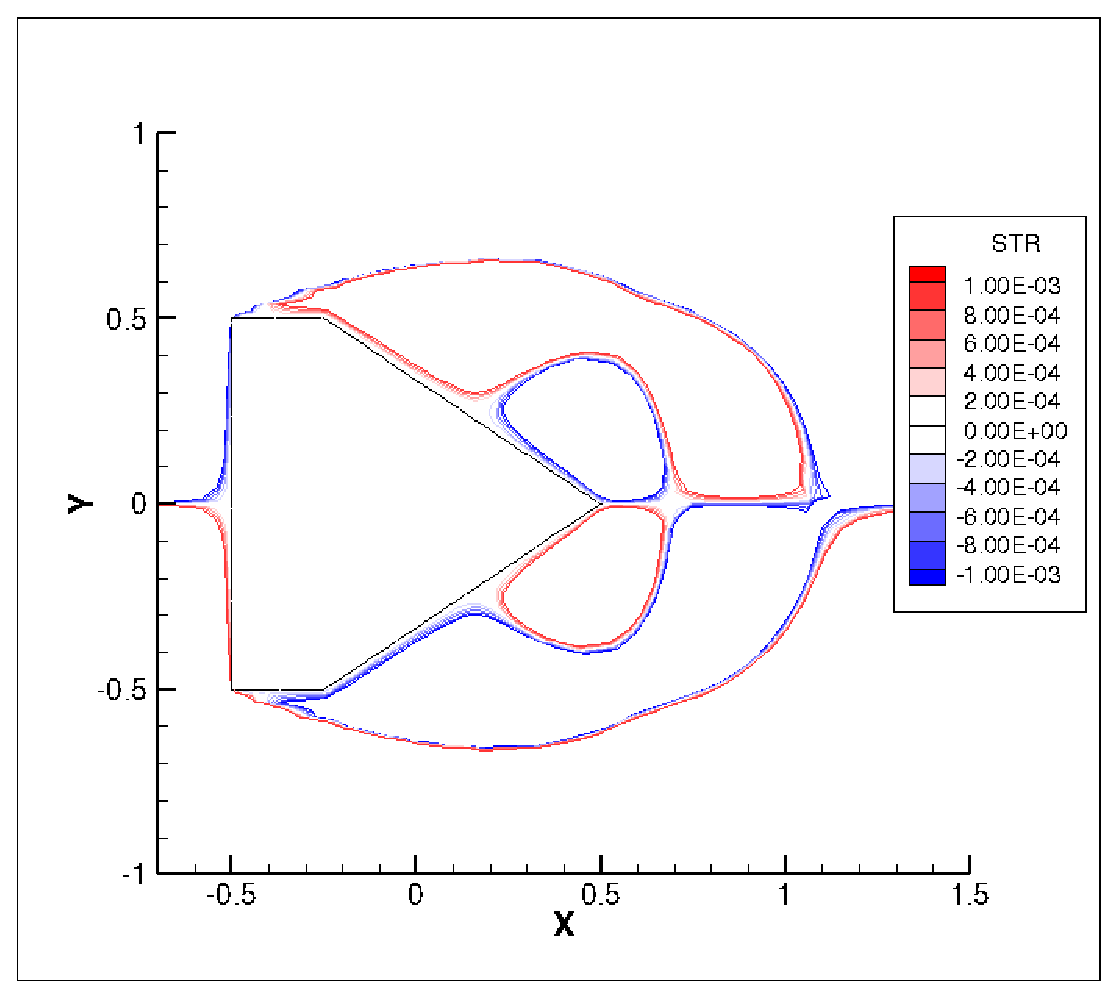
\includegraphics[width=0.4\unitlength]{./chapter-cross-sections/fnp/qss-0.25-3.eps}}
      \put(0.505,0.0){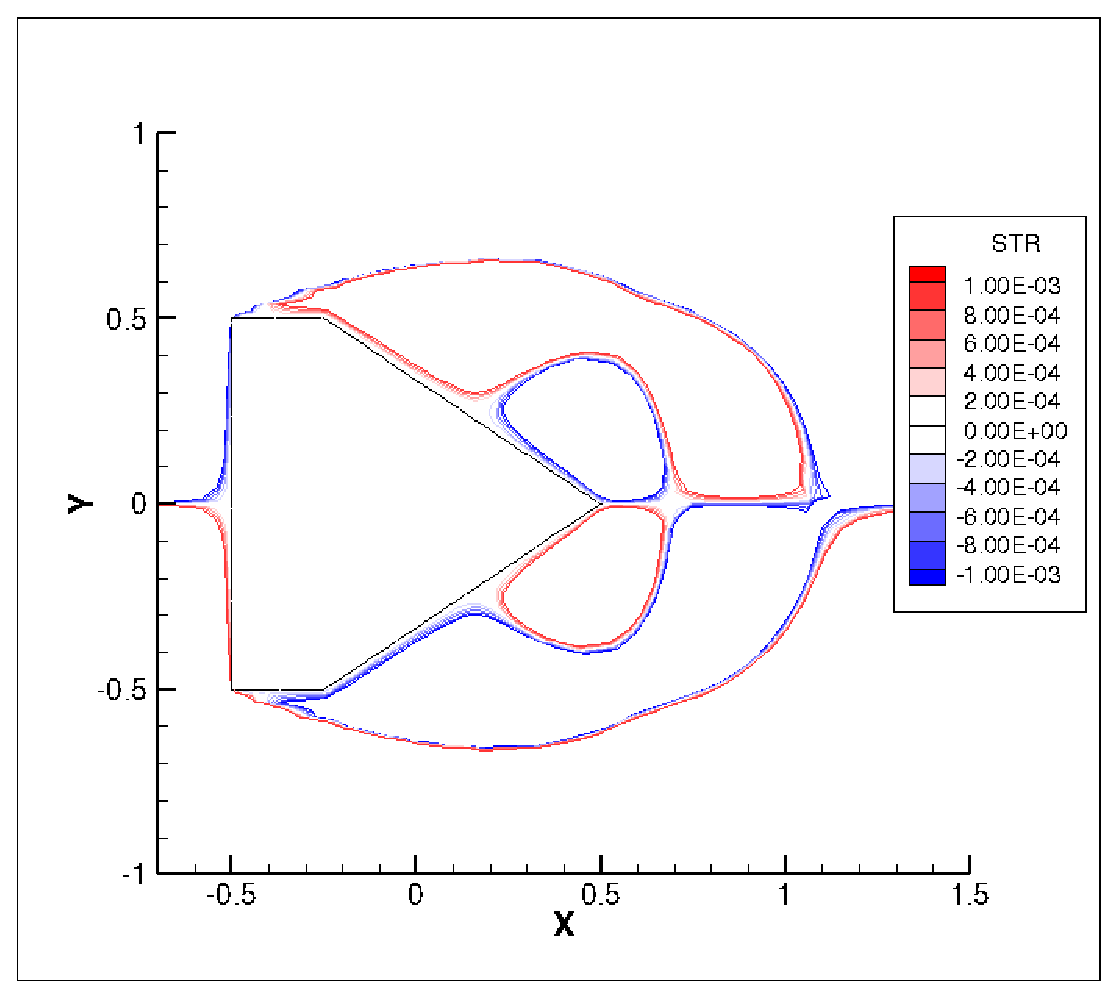
\includegraphics[width=0.4\unitlength]{./chapter-cross-sections/fnp/qss-0.25-3.eps}} 
      
      
%      \put(0.23,0.00){ $\displaystyle\frac{c}{\rho\mathcal{A}U}$}
%      \put(0.73,0.00){ $\displaystyle\frac{c}{\rho\mathcal{A}U}$}


      
      \put(0.01,1.125){\small(a)}
      \put(0.510,1.125){\small(b)}
      \put(0.01,0.725){\small(c)}
      \put(0.510,0.725){\small(d)}
      \put(0.01,0.33){\small(e)}
      \put(0.510,0.33){\small(f)}
      
   
   
      

  \end{picture}

  \caption{Time averaged stream functions of stationary and oscillating flow-fields of the hybrid cross section ($\ratio=0.25$), averaged over a vortex shedding cycle. (a), (c) and (e) the averaged stream functions of the oscillating case at $t=2295.763$ (point 1), $t=2305.897$ (point 2) and $t=2325.870$ (point 3) . (b), (d) and (f) are the stream functions of the flow field of the stationary body corresponding to the induced angles of (a), (c) and (e).\KJ{Justin I cant place this figure where I want to place eventhough I use !h can you have a look please}}  
  \label{fig:flow_field_FSI}
\end{figure}